\section{Introducción al SLAM\textit{(Simultaneous Localization and Mapping)}}
¿Qué cojones es el SLAM?

\subsection{\textit{RTAB-Map SLAM}}
RTAB-Map \textit{(Real-Time Appearance-Based Mapping)} es una técnica de Graph-SLAM\footnote{http://robots.stanford.edu/papers/thrun.graphslam.pdf} basada en la detección de bucles cerrados incrementales. Es totalmente funcional 
con sensores RGB-D, Stereo y LIDAR. \\
El detector de bucles cerrados se basará en la comparativa de cuán semenjantes son la imagenes en una localización y la previa. Cuándo una hipótesis 
de bucle cerrado es aceptada, se añade una nueva restricción al \textit{graph} del mapa y, tras ello, el optimizador minimiza el error del mapa. \\

\begin{figure}[h!]
    \centering
    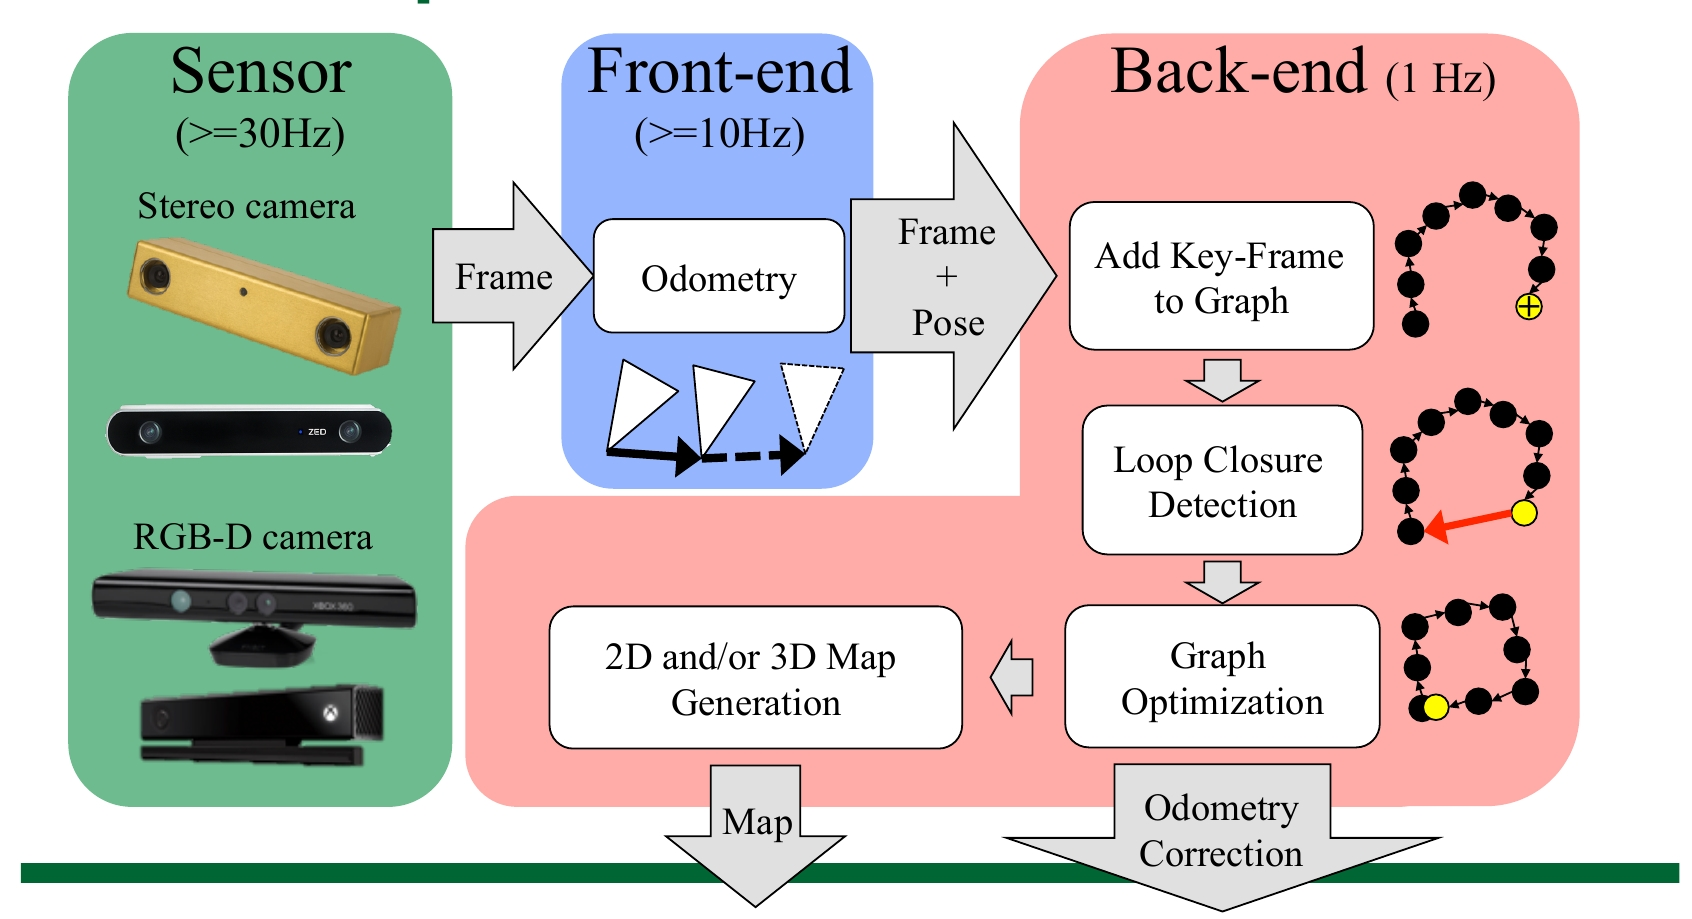
\includegraphics[width=.7\textwidth]{images/rtabmap_scheme}
    \caption{Esquema del Back-End y Front-End de RTAB-Map}
\end{figure}


\subsubsection{Fundamento teórico de la técnica}
Este algoritmo plantea una estrategia de particionado de memoria que pretende asemejarse al funcionamiento de la memoria humana, 
dónde ésta se estructura en: \\
Memoria de trabajo del robot \textit{(Working Memory)}, la memoria a largo plazo \textit{(Long Term Memory)}, 
la memoria a corto plazo \textit{(Short-term memory)} y la memoria sensorial \textit{(Sensory Memory)}. \\
De ese modo, se mantendrán en la memoria de trabajo del robot aquellas localizaciones que se han visitado recientemente 
y con más frecuencia, mientras que el resto pasarán a la memoria de largo plazo. \\

\begin{figure}[h!]
    \centering
    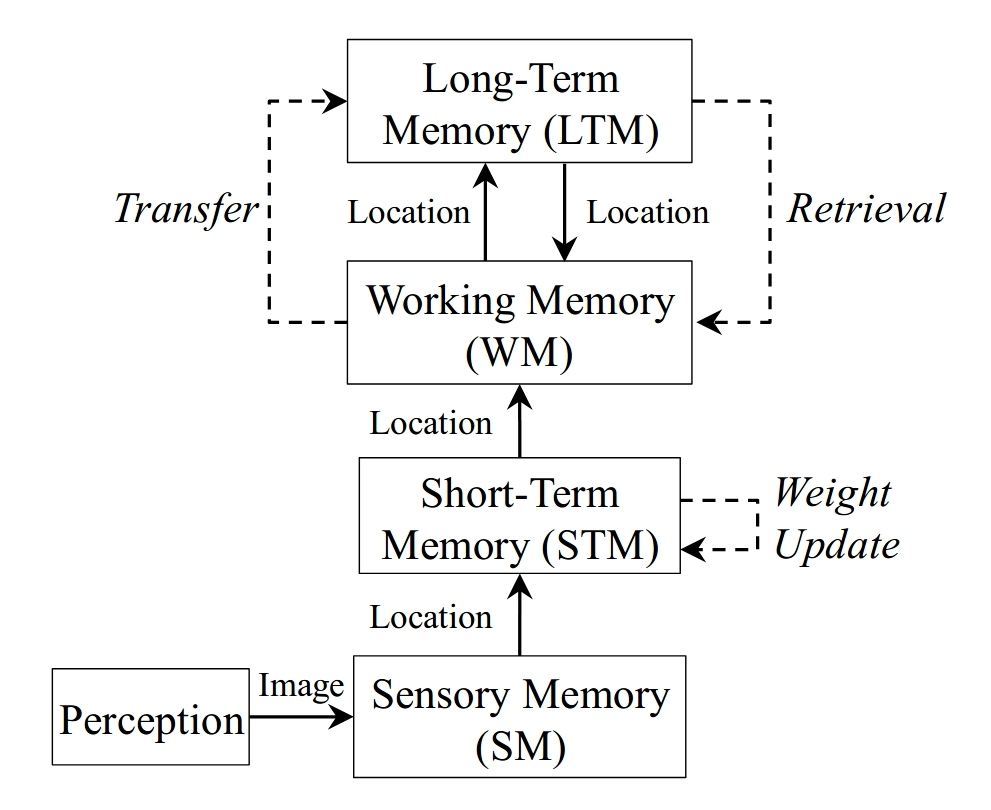
\includegraphics[width=.4\textwidth]{images/rtabmap_memory}
    \caption{Estructura de memoria de la ténica RTAB-Map}
\end{figure}


Se partirá de la premisa de que aquellas localizaciones que son visitadas de forma más frecuente son más propensas a 
crear bucles cerrados. Por ello, el número de veces que una localización sea visitada será empleado como peso, de 
esta forma serán transferidas desde la memoria de trabajo a la memoria de largo plazo aquellas observaciones que 
tengan mayor peso.\\
La memoria a corto plazo, \textit{STM}, tiene como misión buscar las similitudes que existan entre dos imágenes
consecutivas, mientras que la memoria de trabajo, \textit{WM}, es la encargada de detectar los bucles cerrados entre las
localizaciones en el espacio. El número de localizaciones almacenadas en la memoria del trabajo del robot es
limitado. El tamaño de la memoria a corto plazo, \textit{STM}, está basado en la velocidad del robot y en la frecuencia de
adquisición de las localizaciones. \\

% NO SE SI METER ESTA PARTE
\begin{comment}
Es importante destacar que todas las observaciones almacenadas en la memoria a largo plazo, \textit{STM}, del robot no se
usan para detectar bucles cerrados. No obstante, es importante elegir cuidadosamente las localizaciones que se
almacenan en esta memoria. Almacenar las observaciones según la técnica FIFO (First In First Out), sería un
error debido a que, como el algoritmo establece un número máximo de localizaciones que se pueden
almacenar mientras se está explorando un entorno, podríamos alcanzar el superar el umbral de tiempo
establecido sin llegar a cerrar el bucle haciendo que las localizaciones más antiguas nunca consigan asociarse. \\
Como alternativa, el orden de almacenamiento de las observaciones se elige de forma aleatoria, aunque es
preferible mantener en la memoria de trabajo aquellas localizaciones que son más susceptibles de ser
observadas.
\end{comment}
\subsubsection{Análisis de resultados obtenidos}

\subsection{\textit{ORB-SLAM 2}}
\subsubsection{Fundamento teórico de la técnica}
\subsubsection{Análisis de resultados obtenidos}